\subsection{Newton Basis Functions}
Consider a set of data points $\{(x_i, y_i)\}_{i=0}^n$. The \textbf{Newton basis functions} $\left\{n_j(x)\right\}_{j=0}^n$ are the $j$-th order polynomials defined as follows,
\[n_j(x)=\prod_{k=0}^{j-1}\left(x-x_k\right)\]
The resulting linear system for interpolation is,
\[
\left(\begin{array}{cccc}
1 & 0 & \ldots & 0 \\
1 & x_1-x_0 & & 0 \\
1 & x_2-x_0 & & 0 \\
\vdots & \vdots & \ddots & \vdots \\
1 & x_n-x_0 & \ldots & \prod_{k=0}^{n-1}\left(x_n-x_k\right)
\end{array}\right) \left(\begin{array}{c}
c_0 \\
c_1 \\
c_2 \\
\vdots \\
c_n
\end{array}\right)=\left(\begin{array}{c}
y_0 \\
y_1 \\
y_2 \\
\vdots \\
y_n
\end{array}\right)
\]
and, as with Lagrange interpolation, it is \textbf{well-conditioned}.

\begin{rmk}
    This matrix is lower triangular, so we can use \textbf{forward substitution} to find the coefficients $c_j$.
    \begin{align*}
        &c_0=y_0=: f\left[x_0\right] \\
        &c_1=\frac{y_1-c_0}{x_1-x_0}=\frac{y_1-y_0}{x_1-x_0}=\frac{f\left[x_1\right]-f\left[x_0\right]}{x_1-x_0}=: f\left[x_0, x_1\right] \\
        &c_2=\frac{1}{x_2-x_1}\left(f\left[x_0, x_2\right]-f\left[x_0, x_1\right]\right)=: f\left[x_1, x_0, x_2\right]=f\left[x_0, x_1, x_2\right]
    \end{align*}
\end{rmk}

\begin{defn}[Newton's Divided Differences]
    Given a set of data points $\{(x_i, y_i)\}_{i=0}^n$, the $k$-th order \textbf{divided difference} of $f$ is,
    \[
    \begin{array}{ll}
        k=0: & f\left[x_i\right]:=y_i \\
        k>0: & f\left[x_i, \ldots, x_{i+k}\right]:=\frac{f\left[x_{i+1}, \ldots, x_{i+k}\right]-f\left[x_i, \ldots, x_{i+k-1}\right]}{x_{i+k}-x_i}
    \end{array}
    \]
\end{defn}

\begin{ex}{Newton's Divided Differences}{label}
Fix $x_0$, $x_1$, and $x_2$. Then,
\begin{align*}
    f\left[x_0, x_1\right] &=\frac{y_1-y_0}{x_1-x_0} \\
    f\left[x_0, x_1, x_2\right] &=\frac{f\left[x_1, x_2\right]-f\left[x_0, x_1\right]}{x_2-x_0}=\frac{\frac{y_2-y_1}{x_2-x_1}-\frac{y_1-y_0}{x_1-x_0}}{x_2-x_0}
\end{align*}
\end{ex}

\begin{marginfigure}
    It can be shown that $f[x_{\sigma(1)}, x_{\sigma(2)}, \ldots, x_{\sigma(n)}]$ is equal to $f\left[x_0, x_1, \ldots, x_n\right]$ for any permutation $\sigma:\{0, \ldots, n\} \rightarrow\{0, \ldots n\}$. Thus, we can always reorder the arguments with increasing indices.
\end{marginfigure}

\begin{rmk}
    By induction on forward substitution, it can shown that the coefficients $c_j$ in Newton basis are just $f\left[x_0, \ldots, x_j\right]$
\end{rmk}

\begin{thm}[Newton's Divided Difference Interpolation Formula]
    Given a set of data points $\{(x_i, y_i)\}_{i=0}^n$, the polynomial interpolation can be expressed using the Newton basis as,
    \begin{align*}
    f_n(x)
    &=f\left[x_0\right]+\sum_{k=1}^n f\left[x_0, \ldots, x_k\right] \prod_{i=0}^{k-1}\left(x-x_i\right) \\
    &= f_{n-1}(x)+f\left[x_0, \ldots, x_n\right] \prod_{i=0}^{n-1}\left(x-x_i\right)
    \end{align*}
\end{thm}

\begin{marginfigure}
    The second statement of Newton's Divided Difference Interpolation Formula can be useful if additional data points are added incrementally.
\end{marginfigure}

\begin{ex}{Revisiting our Lagrange Interpolation Example}{label}
     Given $\{(0,5),(1,4),(3,-2)\}$, we found that
     \[f_2(x)=\frac{1}{3}\left(-2 x^2-x+15\right)\]
     If we add one data point $(6, 1)$, then $f_3(x)$ can be easily computed using Newton's Divided Difference Interpolation Formula. We need only compute $f[0, 1, 3, 6]$:
     \begin{align*}
     f_3(x)
     &=f_2(x)+f[0,1,3,6](x-0)(x-1)(x-3) \\
     &=\frac{11}{45} x^3-\frac{74}{45} x^2+\frac{18}{45} x+5
     \end{align*}
     To do this, we will maintain a table:
    \begin{center}
    
\includegraphics[width=\textwidth]{figures/fig-12.png}
    \end{center}
\end{ex}

\begin{marginfigure}
    Lagrange and Newton basis functions are preferred because they are well-conditioned, but all three interpolation methods give the same polynomial satisfying $f_n(x_i) = y_i$ for all $0 \leq i \leq n$.
\end{marginfigure}

\subsection{Error Analysis}
We want to \textbf{quantify how well} $f_n(x)$ approximates $f(x)$ on the interval $[a, b]$. This error depends on the choice of $\{x_0, x_1, \cdots, x_n\}$, as well as the derivatives of $f$, and it is captured by the following theorem.

\begin{lem}[Generalized Rolle's Theorem]
    If \text{$g \in C^{n+1}([a, b])$} and $g = 0$ on $n + 2$ distinct points $\left\{x_0, \ldots, x_n, x_{n+1}\right\}$ in $[a,b]$, then $\exists \xi$ between two points in $\left\{x_0, \ldots, x_n, x_{n+1}\right\}$ so that $g^{(n+1)}(\xi) = 0$.
\end{lem}

\begin{thm}[Lagrange Interpolation Error]
    Let $f \in C^{n+1}([a,b])$. Fix $x_1, \cdots x_n \in [a,b]$. For all $x \in [a,b]$, $\exists \xi(x) \in(a, b)$ so that,
    \[f(x)=f_n(x)+\underbrace{\frac{f^{(n+1)}(\xi(x))}{(n+1) !}\left(x-x_0\right) \cdots\left(x-x_n\right)}_{\texttt{Error}}\]
\end{thm}

\begin{proof}
    Let $x \in [a,b]$. If $x = x_i$ for all $i \in [n]$, then $f(x_i) = f_n(x_i) + 0$ and the statement holds. Assume that this is not the case.
    \begin{enumerate}
        \item \textbf{(Step 1)} Construct a function $g$ with $n + 2$ distinct roots using $f$ and $f_n$. For fixed $x \in [a,b]$ and a dummy variable $t$,
        \[g(t):=f(t)-f_n(t)-\left(f(x)-f_n(x)\right) \underbrace{\frac{\left(t-x_0\right) \cdots\left(t-x_n\right)}{\left(x-x_0\right) \cdots\left(x-x_n\right)}}_{\texttt {Denominator} \neq 0}\]
        \item \textbf{(Step 2)} If $t = x_i$, then for any $i \in [n]$, we have that,
        \[g\left(x_i\right)=f\left(x_i\right)-f_n\left(x_i\right)-\left(f(x)-f_n(x)\right) \times 0\]
        Moreover, if $t = x$, then,
        \[g(x)=f(x)-f_n(x)-\left(f(x)-f_n(x)\right) \times 1\]
        That is, \text{$g = 0$} on \text{$n + 2$} distinct points $\left\{x_0, \ldots, x_n, x\right\}$. By the generalized Rolle's Theorem, $g^{(n+1)}(\xi(x))=0$ for some $\xi(x)$.
        \item \textbf{(Step 3)} Computing $g^{(n+1)}(t)$,
        \begin{align*}
            g^{(n+1)}(t)=& f^{(n+1)}(t)-f_n^{(n+1)}(t) \\
            &-\left(f(x)-f_n(x)\right) \frac{d^{(n+1)}}{d t^{(n+1)}}\left(\frac{\left(t-x_0\right) \cdots\left(t-x_n\right)}{\left(x-x_0\right) \cdots\left(x-x_n\right)}\right)
            \end{align*}
            and simplifying at $t = \xi(x)$ gives,
            \begin{align*}
                0 &= g^{(n+1)}(\xi(x)) \\
              &=f^{(n+1)}(\xi(x))-\left(f(x)-f_n(x)\right) \frac{(n+1) !}{\left(x-x_0\right) \cdots\left(x-x_n\right)}
            \end{align*}
            which can be re-arranged to obtain the result,
            \[f(x)=f_n(x)+\frac{f^{(n+1)}(\xi(x))}{(n+1) !}\left(x-x_0\right) \cdots\left(x-x_n\right)\]
    \end{enumerate}
\end{proof}

\begin{cor}
     We can bound the error as follows,
     \begin{align*}
        \left|f(x)-f_n(x)\right| &=\left|\frac{f^{(n+1)}(\xi(x))}{(n+1) !}\left(x-x_0\right) \cdots\left(x-x_n\right)\right| \\
        & \leq \frac{M_{n+1}}{(n+1) !} \max _{x \in[a, b]}\left|\left(x-x_0\right) \cdots\left(x-x_n\right)\right|
    \end{align*}
    since $\left|f^{(n+1)}(\xi(x))\right| \leq \max _{x \in[a, b]}\left|f^{(n+1)}(x)\right|=: M_{n+1}$.
\end{cor}
    
\begin{rmk}
    If $f$ is a polynomial of degree less than or equal to $n$, i.e., $f^{(n+1)}(x)=0$, then the interpolation is exact.
\end{rmk}

\begin{marginfigure}
    In general, the value of $M_{n+1}$ depends on how fast $f$ is changing on the interval $[a,b]$. The product terms of the upper bound will depend on how $\{x_0, \cdots, x_n\}$ are chosen on $[a,b]$.
    \begin{center}
        
\includegraphics[width=\textwidth]{figures/fig-13.png}
        
\includegraphics[width=\textwidth]{figures/fig-14.png}
        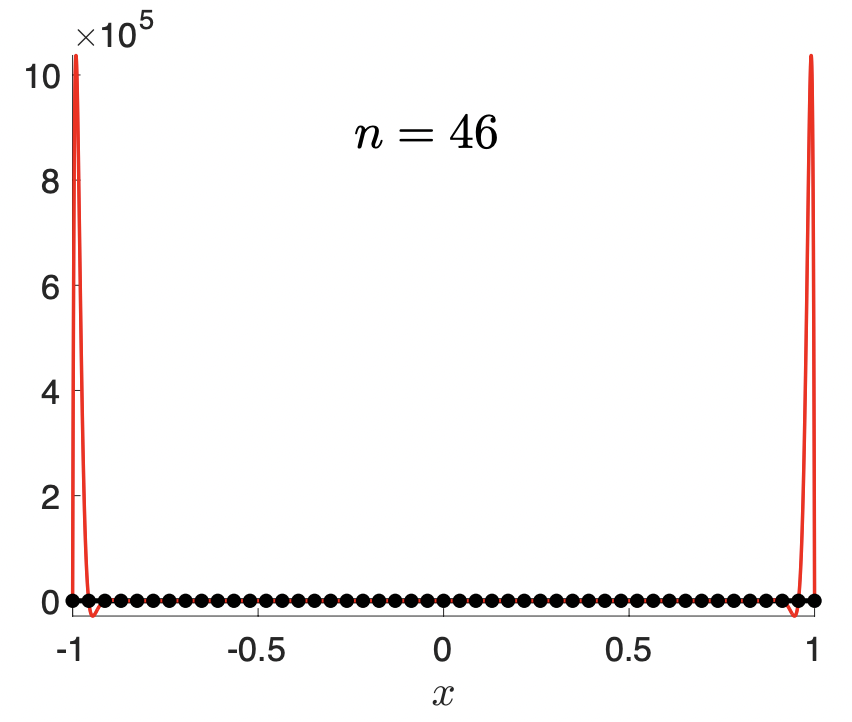
\includegraphics[width=\textwidth]{figures/fig-15.png}
    \end{center}
\end{marginfigure}

\noindent For a fixed function $f$, we want to pick $\{x_0, \cdots, x_n\}$ to minimize the error. A natural choice is to select points with a \textbf{uniform spacing} $h := \frac{b-a}{n}$. Specifically, we will define $x_i := a + ih$ for $i \in [n]$. 

\begin{thm}[Error Bound for Uniformly-Spaced Points]
    \[\left|f(x)-f_n(x)\right| \leq M_{n+1} \frac{h^{n+1}}{4(n+1)}=\frac{M_{n+1}(b-a)^{n+1}}{4 n^{n+1}(n+1)}\]
\end{thm}

\begin{proof}
    The proof is left as an exercise on Assignment 2.
\end{proof}

\subsection{Runge's Phenomenon}
High degree interpolation does not always imply high accuracy. Consider the function $f(x)=1/(1+25 x^2)$ on $[-1,1]$ shown in the margin. There exist some $x \in (-1,1)$ such that $\lim _{n \rightarrow \infty}\left|f(z)-f_n(z)\right|=\infty$. We will formulate a minimization problem that allows us to interpolate on points with \textbf{non-uniform spacing}. We want to minimize,
\[\max _{x \in[a, b]}|\underbrace{\left(x-x_0\right) \cdots\left(x-x_n\right)}_{=x^{n+1}+a_n x^n+\cdots+a_0}|\]
since we have no control over $M_{n+1}$. Write,
\[\mathbb{P}_n=\left\{p(x)=a_n x^n+\cdots+a_0: a_i \in \mathbb{R}\right\}\]
for the set of all polynomials of degree $n$ with real coefficients, and,
\[\tilde{\mathbb{P}}_n=\left\{p(x) \in \mathbb{P}_n: a_n=1\right\}\]
for the set of all \textbf{monic} polynomials of degree $n$. Let
\[\left(x-x_0\right) \cdots\left(x-x_n\right) \in \tilde{\mathbb{P}}_{n+1}\]
and consider the interval $[-1,1]$, which we can transform to $[a,b]$ via
\[x:=\frac{(b-a) t+(b+a)}{2} \in[a, b]\]
for $t \in[-1,1]$. We want to find $\tilde{q}(t) \in \tilde{\mathbb{P}}_{n+1}$ so that
\[\max _{t \in[-1,1]}|\tilde{q}(t)| \leq \max _{t \in[-1,1]}|\tilde{p}(t)| \quad \quad (\star)\]
for all $\tilde{p}(t) \in \tilde{\mathbb{P}}_{n+1}$. The unique monic polynomial solving our minimization problem $(\star)$ is defined by the roots of the polynomial:

\begin{marginfigure}
    $(\star)$ is called the \textbf{optimal monic polynomial problem}, and the unique monic polynomial that solves it is the \textbf{Chebyshev polynomial}.
\end{marginfigure}

\begin{defn}[Chebyshev Polynomial]
    \sloppy The \textbf{Chebyshev polynomial} $T_n$ is the $n$-th degree polynomial defined on $[-1,1]$ by,
    \[T_n(t)=\cos (n \arccos (t))\]
\end{defn}

\begin{marginfigure}
Recall the cosine angle sum identities,
\begin{align*}
&\sin (\alpha+\beta)=\sin \alpha \cos \beta+\cos \alpha \sin \beta \\
&\cos (\alpha+\beta)=\cos \alpha \cos \beta-\sin \alpha \sin \beta \\
&\sin (\alpha-\beta)=\sin \alpha \cos \beta-\cos \alpha \sin \beta \\
&\cos (\alpha-\beta)=\cos \alpha \cos \beta+\sin \alpha \sin \beta
\end{align*}
\end{marginfigure}

\begin{rmk}
    Computing $T_n$ for $n = 0, 1, 2$,
    \begin{align*}
    &T_0(t)=\cos (0)=1 \\
    &T_1(t)=\cos (\arccos (t))=t \\
    &T_2(t)=\cos (2 \underbrace{\arccos (t)}_{\theta})=\cos (2 \theta)=2 \cos ^2 \theta-1=2 t^2-1
    \end{align*}
    where the result for $T_n$ follows by trigonometric identities. With $T_0$ constant, this gives the following recurrence relation,
    \[T_2(t)=2 t T_1(t)-T_0(t)\]
    which, by induction, generalizes to,
    \begin{align*}
    T_{n+1}(t) &=2 t T_n(t)-T_{n-1}(t) \\
    & \in 2 t\left(2^{n-1} t^n+\mathbb{P}_{n-2}\right)+\mathbb{P}_{n-1} \subset 2^n t^{n+1}+\mathbb{P}_{n-1}
    \end{align*}
\end{rmk}

\begin{rmk}
    The zeroes of $T_{n+1}$ are,
    \[t_k=\cos \left(\frac{(2 k+1) \pi}{2(n+1)}\right) \quad k = 0, 1, \cdots, n\]
    The extremal points $T_{n+1}$ are,
    \[z_k=\cos \left(\frac{k \pi}{n+1}\right)\quad k = 0, 1, \cdots, n+1\]
    with values $T_{n+1}\left(z_k\right)=(-1)^k$.
\end{rmk}

\begin{marginfigure}
\begin{center}
       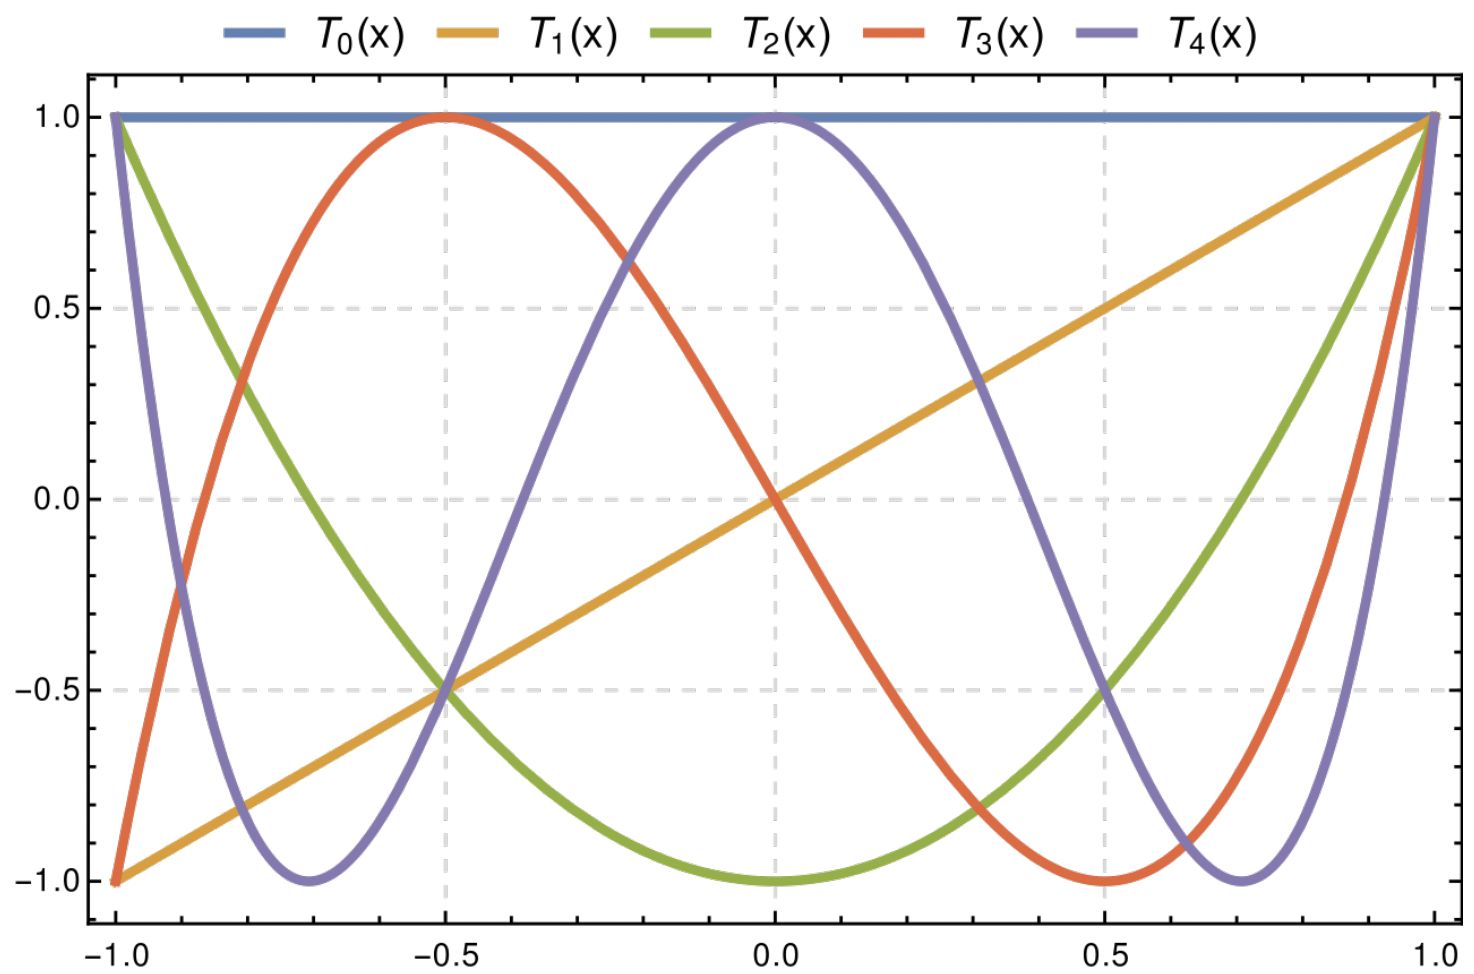
\includegraphics[width=\textwidth]{figures/fig-5.png}
\end{center}
\end{marginfigure}

\begin{thm}[Chebyshev Equioscillation]
    The polynomial,
    \[\frac{T_{n+1}(t)}{2^n}\]
    is the unique monic polynomial that solves our minimization problem $(\star)$. Specifically, for any $\tilde{p}_{n+1}(x) \in \tilde{\mathbb{P}}_{n+1}$, 
    \[\frac{1}{2^n}=\max _{t \in[-1,1]}\left|\frac{T_{n+1}(t)}{2^n}\right| \leq \max _{t \in[-1,1]}\left|\tilde{p}_{n+1}(t)\right|\]
\end{thm}

\begin{proof}
    Assume that there exists another monic polynomial,
    \[\tilde{p}_{n+1}(x) \neq \frac{T_{n+1}(t)}{2 n}\]
    with a smaller maximum absolute value,
    \[\max _{t \in[-1,1]}\left|\tilde{p}_{n+1}(t)\right|<\max _{t \in[-1,1]}\left|\frac{T_{n+1}(t)}{2^n}\right|=\frac{1}{2^n}\]
    Define a polynomial $Q(t)$ as follows,
    \[Q(t):=\frac{T_{n+1}(t)}{2^n}-\tilde{p}_{n+1}(t)\]
    $T_{n+1}$ and $\tilde{p}_{n+1}$ have \text{$a_{n+1}=1$}, so $Q(t)$ is a polynomial of order $n$. Evaluating $Q$ on all extremal points $z_k$ of $T_{n+1}$ for all \textbf{$k \in [n+1]$},
    \[
    Q\left(z_k\right)=\frac{(-1)^k}{2^n}-\tilde{p}_{n+1}\left(z_k\right)\left\{\begin{array}{c}
    \geq \frac{1}{2^n}-\left|\tilde{p}_{n+1}\left(z_k\right)\right|>0, \text { if } k \text { even} \\
    \leq-\frac{1}{2^n}+\left|\tilde{p}_{n+1}\left(z_k\right)\right|<0, \text { if } k \text { odd}
    \end{array}\right.
    \]
    By the Intermediate Value Theorem, it follows that $Q(t)$ has a zero between $\left[z_k, z_{k+1}\right]$ for \text{$k = 0, \cdots, n$}. This implies that $Q(t)$ has \text{$n + 1$} distinct zeroes, and consequently that $Q(t)$ must be the zero polynomial (since $Q(t)$ is of degree $n$). Thus,
    \[\tilde{p}_{n+1}(t)=\frac{T_{n+1}(t)}{2^n}\]
\end{proof}

\begin{marginfigure}
Returning to our previous example, we see that interpolating on,
\[t_k=\cos \left(\frac{(2 k+1) \pi}{2(n+1)}\right)\]
produces a polynomial interpolant with no unbounded oscillations.
\end{marginfigure}